\subsection{MEX 2-2: Closure and healing of cracks (IfG)}

Participating institutions of MEX 2-2 (see section \ref{sec:mex03}): IfG, UFZ

The measured gas flow is converted into permeabilities, which are stored as time series in an Excel file. For each of the three experiment there are two columns. The first contains the time in hours since the start of the experiment, the second contains the permeability. 

\begin{figure}[!ht]
\centering
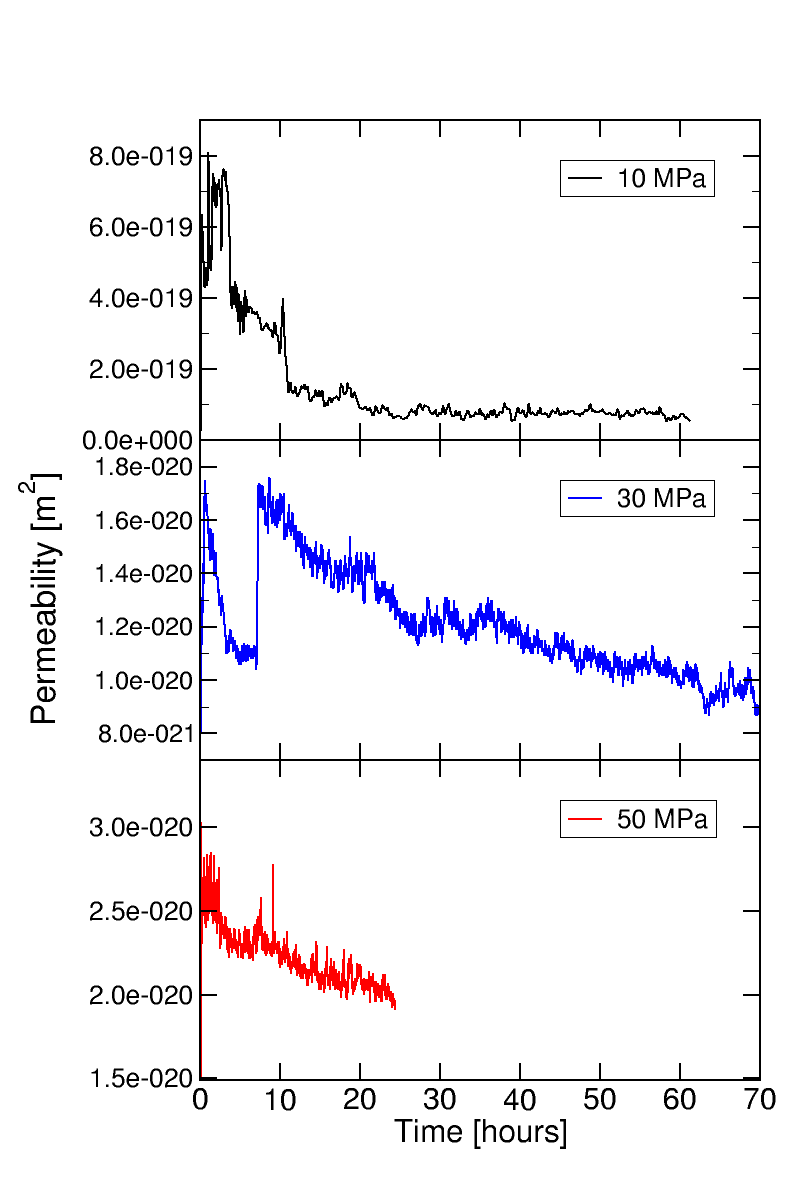
\includegraphics[width=0.75\textwidth]{figures/mex3-perme-time-comparison.png}
\caption{Graphical Representation of data.}
\label{fig:ME3-perme-exp-dmp}
\end{figure}

\begin{table}[!ht]
\caption{MEX 2-2: Meta Data according to Dublin Core}
\label{tab:dms-mex2-2}
\small
\begin{tabular}{R{3cm}|L{7cm}}
\hline
%
Data label &  \\
URI &  \\
Subject  &  \\
Type of data  &  \\
Dataquality  &  \\
Status of data  &  \\
Dataformat  & \\
Creators  &  \\
Source/Origin &  \\
Publisher  &  \\
Rights holders &  \\
Contributors &  \\
Time or Period of creation &  \\
Language of the content &  \\
Update policy &  \\
Access permissions &  \\
%
\hline
\end{tabular}
\end{table}